\section*{HS/13. feladat: Hőátszármaztatás síkfalon keresztül}
\addcontentsline{toc}{section}{HS/13. feladat: Hőátszármaztatás síkfalon keresztül}

\begin{tabular}{ | p{2cm} | p{14cm} | } 
	\hline
	Név & Vasáros Mátyás \\ 
	\hline
	Szak & Mechatronikai mérnök\\ 
	\hline
	Félév & 2019/2020 II. (tavaszi) félév \\ 
	\hline
\end{tabular}
\vspace{0.5cm}

\noindent A feladat egy nagy kiterjedésű homogén síkfal stacioner állapotú hőátszármaztatása esetén kiszámítani a hőáramsűrűséget és a fal két oldalán a hőfokesést. A fal két oldalán ismert a hőmérséklet ezek $T_{f1}=\SI{400}{\degreeCelsius}$ és $T_{f2}=\SI{200}{\degreeCelsius}$. A fal egyik oldalán a hőátadási tényező értéke az átváltás után $\alpha_1=\SI{1162}{\watt\per\meter\squared\kelvin}$ a másik oldalon $\alpha_2=\SI{581,5}{\watt\per\meter\squared\kelvin}$, a fal hőátadási tényezője $\lambda=\SI{446,52}{\watt\per\meter\kelvin}$. A fal vastagsága $\delta=\SI {16}{\milli\meter}=\SI {0,016}{\meter}$.

\begin{figure}[h]
	\centering
	\label{figure:vgtsd}
	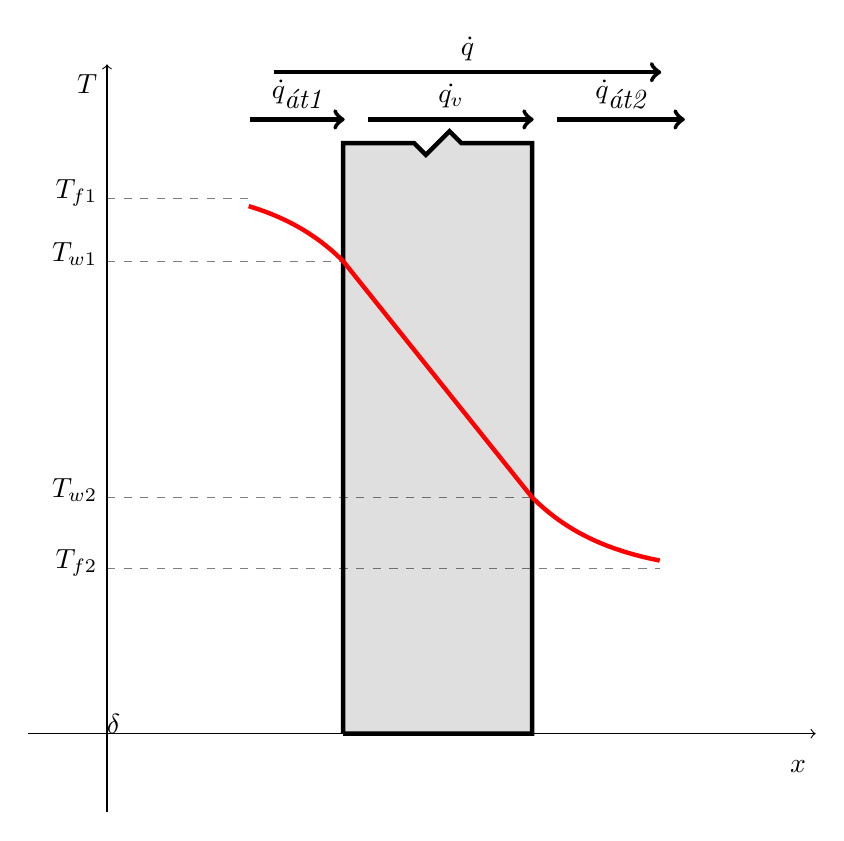
\begin{tikzpicture}
	
	\pgfmathsetmacro{\zoom}{1.5}
	\pgfmathsetmacro{\szel}{6*\zoom}
	\pgfmathsetmacro{\mag}{5*\zoom}
	\pgfmathsetmacro{\fal}{1.6*\zoom}
	\pgfmathsetmacro{\xdis}{2*\zoom}
	

	\pgfmathsetmacro{\Twegy}{4*\zoom}
	\pgfmathsetmacro{\Twketto}{2*\zoom}	

	\pgfmathsetmacro{\et}{\xdis+\fal}
	\pgfmathsetmacro{\von}{0.1*\zoom}
	% Tengelyek
	\draw[->] (0,-1) -- (0,\mag+1) node[anchor=north east]{$T$};
	\draw[->] (-1,0) -- (\szel,0) node[anchor=base east, shift={(0,-0.5)}]{$x$};
	
	%Fal
	\fill[gray,opacity=0.25](\xdis,0) -- (\xdis,\mag) --(\xdis+\fal/2-2*\von ,\mag) --(\xdis+\fal/2-\von ,\mag-\von) --(\xdis+\fal/2+\von ,\mag+\von)--(\xdis+\fal/2+2*\von ,\mag)-- (\et,\mag) -- (\et,0) -- (\xdis,0);
	
	\draw[ultra thick] (\xdis,0) -- (\xdis,\mag) --(\xdis+\fal/2-2*\von ,\mag) --(\xdis+\fal/2-\von ,\mag-\von) --(\xdis+\fal/2+\von ,\mag+\von)--(\xdis+\fal/2+2*\von ,\mag)-- (\et,\mag) -- (\et,0) -- (\xdis,0);
	
	%Szaggatott vonalak/felíratok
	\draw[black, opacity=0.5, dashed] (0,\Twegy+0.8) -- (\xdis*0.6,\Twegy+0.8);
	\node[anchor=base east] at (0,\Twegy+0.8) {$T_{f1}$};		
	\draw[black, opacity=0.5, dashed] (0,\Twegy) -- (\xdis,\Twegy);
	\node[anchor=base east] at (0,\Twegy) {$T_{w1}$};
	\draw[black, opacity=0.5, dashed] (0,\Twketto) -- (\xdis+\fal,\Twketto);
	\node[anchor=base east] at (0,\Twketto) {$T_{w2}$};
	\draw[black, opacity=0.5, dashed] (0,\Twketto-0.9) -- (\et*1.3,\Twketto-0.9);
	\node[anchor=base east] at (0,\Twketto-0.9) {$T_{f2}$};	

	%Hőmérséklet vonalak
	\draw[ultra thick, red](\xdis,\Twegy)--(\xdis+\fal,\Twketto);
	\draw[ultra thick, color=red, domain=\xdis*0.6:\xdis, smooth, variable=\r] plot (\r, {\Twegy+1 - (exp(\r-\xdis))});
	\draw[ultra thick, color=red, domain=\et:\et*1.3, smooth, variable=\r] plot (\r, {\Twketto-1 + (exp(-\r+\et))});
	
	%Méretvonal
	\pgflength[xa=\xdis, ya=0, xb=\xdis+\fal, yb=0,ra={1}]{$\delta$};
	
	% Hőáram és hőáramsűrűség
	\draw[->, ultra thick] (\xdis*0.6-\von,\mag+2*\von ) -- (\xdis-\von,{\mag+2*\von}) node[midway, anchor=south]{$\dot{q}_{\textit{át1}}$} ;
	\draw[->, ultra thick] (\xdis+\von,\mag+2*\von ) -- (\et-\von,{\mag+2*\von}) node[midway, anchor=south]{$\dot{q_v}$} ;
	\draw[->, ultra thick] (\et+\von,\mag+2*\von ) -- (\et*1.3+\von,{\mag+2*\von}) node[midway, anchor=south]{$\dot{q}_{\textit{át2}}$} ;
	\draw[->, ultra thick] (\xdis*0.6+\von,\mag+6*\von ) -- (\et*1.3-\von,{\mag+6*\von}) node[midway, anchor=south]{$\dot{q}$} ;
	
	\end{tikzpicture}
	\caption{Hőmérséklet-hely függvény}
\end{figure}

\noindent A hőáramsűrűség a rendszerben létrejövő hőátadások és hővezetések esetén is megegyezik. 

\begin{equation}\label{elso}
\dot{q}=\dot{q}_{\textit{át1}} =\dot{q_v}=\dot{q}_{\textit{át2}}=\alpha_1 (T_{f1}-T_{w1})= \frac{\lambda_1}{\delta_1} (T_{w1} - T_{w2}) = \alpha_2 (T_{w2}-T_{f2})
\end{equation} 

\noindent A tagokat összevonva a következő összefüggést kapjuk.

\begin{equation}
(T_{f1}-T_{f2})=\dot{q}(\frac{1}{\alpha_1}+\frac{\delta}{\lambda}+\frac{1}{\alpha_2})
\end{equation} 

\noindent Ebből $\dot{q}$-t kifejezve az alábbi egyenletet kapjuk.

\begin{equation}
\dot{q}=\frac{T_{f1}-T_{f2}}{\frac{1}{\alpha_1}+\frac{\delta}{\lambda}+\frac{1}{\alpha_2}}
\end{equation} 

\noindent Ahol a hőátadási tényezőket és hővezetési tényezőt a következő módon vonhatjuk össze.

\begin{equation}
\begin{split}
\kappa=\frac{1}{\frac{1}{\alpha_1}+\frac{\delta}{\lambda}+\frac{1}{\alpha_2}}
=\frac{1}{\frac{1}{\SI{1162}{\watt\per\meter\squared\kelvin}}+\frac{\SI {0,016}{\meter}}{\SI{446,52}{\watt\per\meter\kelvin}}+\frac{1}{\SI{581,5}{\watt\per\meter\squared\kelvin}}}
=\SI{342,04}{\watt\per\meter\squared\kelvin}
\end{split}
\end{equation} 

\noindent A hőáramsűrűség ezután a teljes hőmérséklet különbség és a $\kappa$ szorzataként számítható.

\begin{equation}
\dot{q}=\kappa(T_{f1}-T_{f2})=\SI{342,04}{\watt\per\meter\squared\kelvin}(\SI{400}{\degreeCelsius}-\SI{200}{\degreeCelsius})=\SI{76471,06}{\watt\per\meter\squared}
\end{equation}

\noindent Ismerve a hőáramsűrűség értékét kiszámolhatjuk a hőfokeséseket. Az ehhez szükséges egyenletek kifejezhetőek az \ref{elso} egyenletből.

\begin{equation}
(T_{f1}-T_{w1})=\frac{1}{\alpha_1}\dot{q}=\frac{1}{\SI{1162}{\watt\per\meter\squared\kelvin}}\SI{76471,06}{\watt\per\meter\squared}=\SI{65,75}{\kelvin}=\SI{65,75}{\degreeCelsius}
\end{equation}

\begin{equation}
(T_{w2}-T_{f2})=\frac{1}{\alpha_2}\dot{q}=\frac{1}{\SI{581,5}{\watt\per\meter\squared\kelvin}}\SI{76471,06}{\watt\per\meter\squared}=\SI{131,51}{\kelvin}=\SI{131,51}{\degreeCelsius}
\end{equation}
